\section{Methods}

\subsection{Data}

Data from this project were assembled from XXX projects on leaf spectra and related foliar traits (Table~\ref{tab:projectinfo}).
Most of these datasets are obtained directly from the ECOSIS spectral library (https://ecosis.org/).
Collectively, these data are comprised of XX observations from XX species, and span a wide geographic (Figure~\ref{fig:datamap}) and climatic range (Figure~\ref{fig:dataclimate}).

\begin{table}
    \caption{Project information}
    \centering
    \begin{table}[H]
\centering\begingroup\fontsize{8}{10}\selectfont

\begin{tabular}{l>{\raggedright\arraybackslash}p{25em}rrr}
\toprule
Short name & Long name & Samples & Species & Sites\\
\midrule
ACCP & Accelerated Canopy Chemistry Program (ACCP) & 850 & 46 & 5\\
ANGERS & Angers, France spectra from INRA & 274 & 37 & 1\\
Barnes 2017 & Barnes et al. 2017. Beyond greenness: Detecting temporal changes in photosynthetic capacity with hyperspectral reflectance data. PLoS ONE. & 86 & 1 & 1\\
Cali. Eco. Traits & Fresh Leaf Spectra to Estimate Leaf Traits for California Ecosystems & 261 & 16 & 34\\
Cedar Creek Biodiv. & 2014 Cedar Creek ESR Grassland Biodiversity Experiment: Leaf-level Contact Data: Trait Predictions & 780 & 18 & 1\\
\addlinespace
Corn var. & Spectral Characterization of Multiple Corn Varieties: West Madison Agricultural Station 2014 & 288 & 1 & 1\\
Di Vittorio 2009 & Di Vittorio 2009 & 504 & 2 & 3\\
Hawaii 2000 & Hawaii 2000 vegetation species spectra & 588 & 56 & 48\\
LOPEX & Leaf Optical Properties Experiment (1993) & 66 & 45 & 1\\
Milkweed stress & Common Milkweed Leaf Responses to Water Stress and Elevated Temperature & 735 & 1 & 1\\
\addlinespace
Missoula TS & Missoula Montana lodgepole pine \& big sagebrush time series & 100 & 2 & 4\\
NASA FFT & NASA Forest Functional Types (FFT) & 1369 & 66 & 130\\
NASA HyspIRI & NASA HyspIRI field campaign & 1704 & 38 & 12\\
NGEE Arctic & Next Generation Ecosystem Experiment (NGEE) - Arctic & 614 & 13 & 3\\
NGEE Tropics & Next Generation Ecosystem Experiment (NGEE) - Tropics & 706 & 28 & 1\\
\addlinespace
Pepper K/N & Fresh and Dry Pepper Leaf Spectra with Associated Potassium and Nitrogen Measurements & 119 & 1 & 1\\
PVY solanum & Varietal Discrimination and Detection of PVY in Solanum tuberosum: Hawaii 2014 & 761 & 1 & 1\\
Santa Monica Mtns. & Santa Monica Mountains vegetation species spectra & 353 & 24 & 1\\
Soybean aphid & Productivity and Characterization of Soybean Foliar Traits Under Aphid Pressure & 1131 & 1 & 1\\
Spectral variation & Spectral Variation Between Leaf-level and Canopy-level Measurements & 16 & 1 & 1\\
\addlinespace
Wu 2016 & Wu et al. 2016 New Phytologist canopy traits study & 160 & 17 & 1\\
Yang 2016 & Yang et al. 2016 Remote Sensing of Environment & 497 & 3 & 2\\
\bottomrule
\end{tabular}\endgroup{}
\end{table}

    \label{tab:projectinfo}
\end{table}

\begin{figure}
    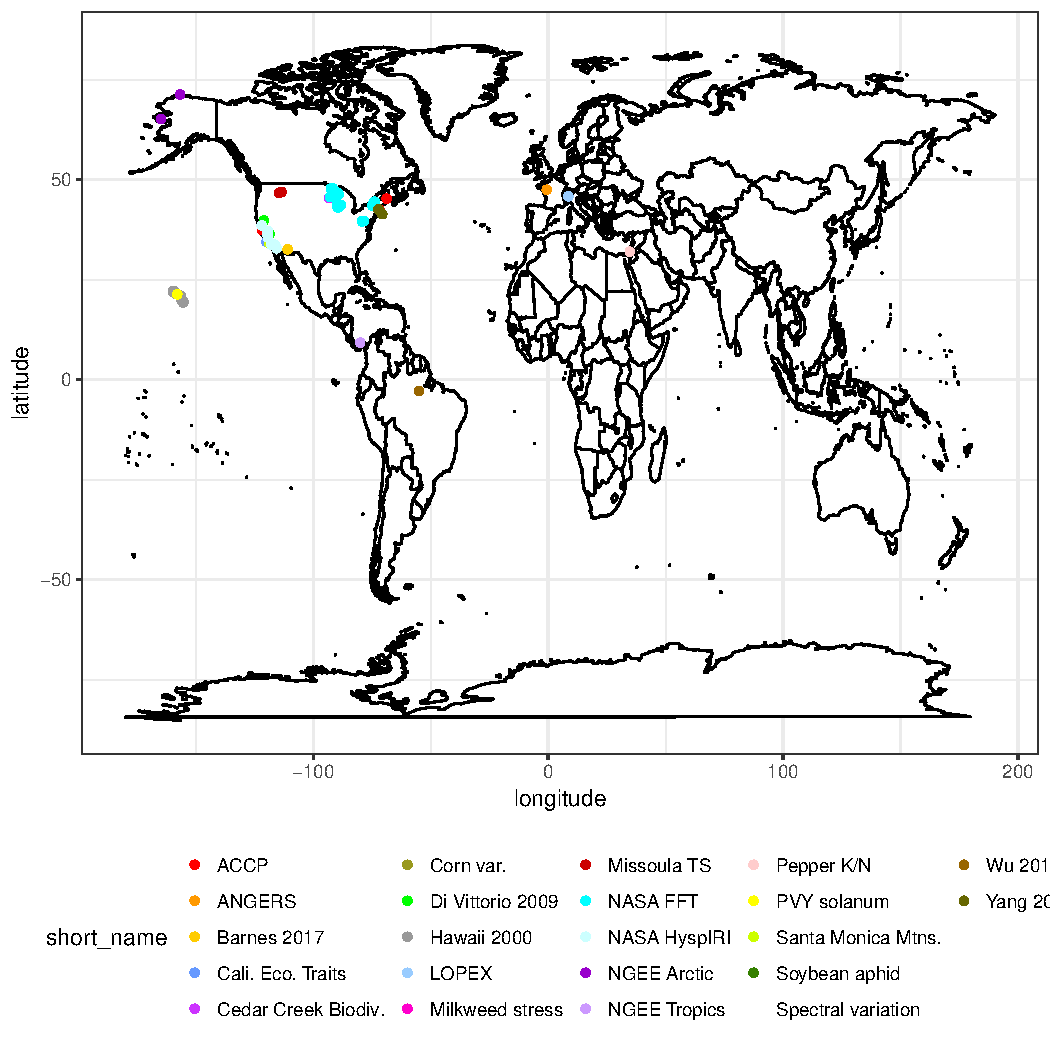
\includegraphics{\string figures/data_map.pdf}
    \caption{Map of data locations}
    \label{fig:datamap}
\end{figure}

\begin{figure}
    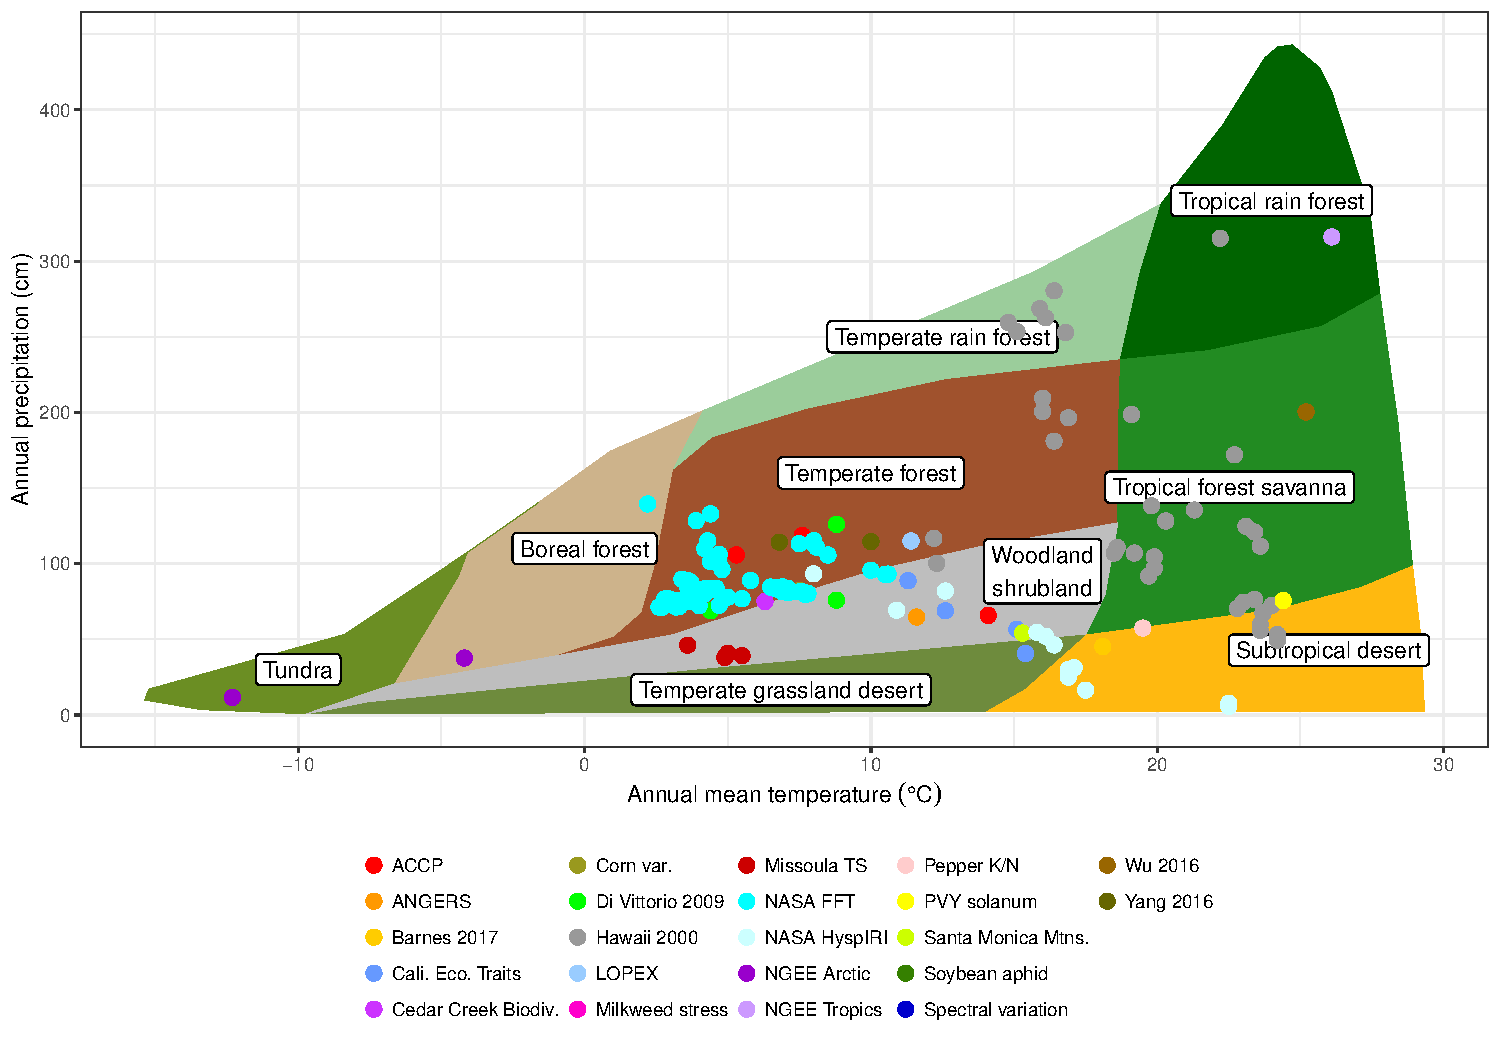
\includegraphics{\string figures/data_climate.pdf}
    \caption{Data locations in climate space}
    \label{fig:dataclimate}
\end{figure}

\subsection{Trait estimation via PROSPECT inversion}

The PROSPECT leaf radiative transfer model \cite{jacquemoud1990_prospect,jacquemoud_2009_prosail,feret2008_prospect,feret2017_prospectd} simulates leaf reflectance and transmittance for 400 to 2500 nm wavelengths at 1 nm increments as a function of leaf morphological and biochemical characteristics.
In this chapter, I compared the performance of four different versions of PROSPECT, each of which uses a different combination of leaf traits:
PROSPECT 4 uses
total chlorophyll content per area ($\mu g ~ cm^{-2}$),
leaf water content per area ($g ~ m^{-2}$),
and leaf dry matter content per area ($g ~ m^{-2}$) \cite{feret2008_prospect}.
PROSPECT 5 extends PROSPECT 4 with a parameter for
total carotenoid content per area ($\mu g ~ cm^{-2}$) \cite{feret2008_prospect}.
PROSPECT 5B adds an additional parameter for
total "senescent brown pigment" content (arbitrary units) \cite{jacquemoud_2009_prosail}.
Finally, PROSPECT D adds an additional parameter for
total anthocynanin content per area ($\mu g ~ cm^{-2}$) \cite{feret2017_prospectd}.

To estimate traits from leaf spectra, we generally followed the Bayesian RTM inversion approach of \cite{shiklomanov2016_rse}, except that we replaced the Metropolis-Hastings algorithm with a more efficient Differential Evolution algorithm with "snooker" update as implemented in the ``BayesianTools'' R package \cite{bayesiantools}.
Forward simulations and Bayesian inversion of PROSPECT are implemented in the R package ``PEcAnRTM'' \cite{shiklomanov2016_rse}, which is open source and freely available at https://github.com/pecanproject/pecan/modules/rtm.
Where leaf spectra extended beyond the 400 to 2500 nm wavelength range of the PROSPECT model, we used only the observations from 400 to 2500 nm.
Where leaf spectra were sampled at a spectral resolution coarser than 1 nm or did not include all wavelengths simulated by PROSPECT, we subset the PROSPECT output in the likelihood function to match the observations.
Where leaf spectra were sampled at a finer spectral resolution than 1 nm, or where wavelengths did not align at 1 nm intervals, we used cubic spline interpolation (default method in the R function `spline`) to align the spectra with PROSPECT output.
Where leaf spectra were provided as ``pseudo-absorbance'' ($1 - \log_{10}(R)$), we added the corresponding transformation to the PROSPECT output in the likelihood calculation. 

\subsection{Analysis}

To compare PROSPECT versions, we plotted traits estimated by more than one version of PROSPECT as pairwise scatter plots, fit a least-squares linear regression to each and compared the result to a 1-to-1 line, and calculated the pairwise correlation coefficient (Figure XXX).
To validate PROSPECT inversions, we compared trait estimates from PROSPECT inversion with direct measurements of the corresponding traits, where these traits were available.
To explore project-specific biases in the inversion, we fit least-squares linear regressions to investigate the ability of trait estimates from spectra to predict the measured traits, and we report the slopes, intercepts, and $R^2$ values of those regressions (Table XXX).
To identify species-specific errors, we also calculated the mean absolute error (MAE) between the measured trait and inversion estimate for each species-project combination (Figure XXX).

To investigate the effects of experimental treatments and environmental conditions, we fit a linear fixed effects model for each optical trait and each treatment, with an additional fixed effect for species if multiple species were present in that treatment.
We then summarized the direction of each GLM coefficient, and whether the coefficient was significant, in a figure (Figure XXX).

%TODO: fill in the rest of the analyses

We performed all analyses using R version 3.4.4 \cite{rstats}.
The data and code for performing these analyses are open source and freely available at https://github.com/ashiklom/rspecan.
